%----------------------------------------------------------------------------
%----------------------------------------------------------------------------
It was observed that the beam profile was asymmetric with respect to the upstream and downstream directions from the waist (see figure \ref{spiricon}).
%----------------------------------------------------------------------------
% spiricon.tex
% by Troy Hix, May 2005
%----------------------------------------------------------------------------
\begin{figure}
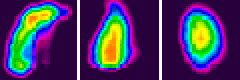
\includegraphics[width=6.00in]
{spiricon/spiricon.png}\\
\caption[Transverse beam profiles from Spiricon camera]{Transverse beam profiles from Spiricon camera. The center image was taken at the apparent waist (downstream from the 2 m lens), the left image was taken 12 inches downstream from the apparent waist, the right image was taken 12 inches upstream from the apparent waist.}
\label{spiricon}
\end{figure} 
%----------------------------------------------------------------------------

%----------------------------------------------------------------------------
As a check, we obtain a similar set of beam profiles using a superposition of the first 4 modes in the Hermite-Gauss expansion. The complex amplitude for the Hermite-Gauss beam is \cite{Siegman:1986a}
%----------------------------------------------------------------------------
%----------------------------------------------------------------------------
%----------------------------------------------------------------------------
\begin{equation}
U_{\ell,m}(x,y,z)
=
A_{\ell,m}
\cdot
\frac{\sqrt{2}}{2^{m+\ell}m!\ell!}
\cdot
\frac
{w_0}
{w(z)}
\cdot
G_{\ell}
\left(
\frac
{\sqrt{2}x}
{w(z)}
\right)
\cdot
G_{m}
\left(
\frac
{\sqrt{2}y}
{w(z)}
\right)
\cdot
\Phi(x,y,z)
\end{equation}
%----------------------------------------------------------------------------
where
%----------------------------------------------------------------------------
\begin{equation}
\Phi(x,y,z)
=
\exp{
\left(
-ikz
-
ik\frac{x^2+y^2}{2R(z)}
+
i(\ell+m+1)
\zeta(z)
\right)
},
\end{equation}
%----------------------------------------------------------------------------
\begin{equation}
G_n(u)
=
H_n(u)
\exp
\left(
\frac
{-u^2}
{2}
\right),
\quad
n=0,1,2\ldots,
\end{equation}
%----------------------------------------------------------------------------
\begin{equation}
\zeta(z)
=
\arctan
\left(
\frac{z}{z_0}
\right),
\end{equation}
%----------------------------------------------------------------------------
$H_n(u)$ is the nth Hermite polynomial, and $A_{\ell,m}$ are the complex expansion coefficients.

It was found with some trial and error that the following set of expansion coefficients generated a composite beam which has a similar profile to the raw dye laser beam as seen on the Spiricon camera:
%----------------------------------------------------------------------------
\begin{eqnarray}
A_{0,0} &=& 5\exp{(-i0.02\pi)}\\
A_{0,1} &=& 1.4\exp{(i0.4\pi)}\\
A_{1,0} &=& 1.8\exp{(i1.6\pi)}\\
A_{1,1} &=& 1.5\exp{(i0.5\pi)},
\end{eqnarray}
%----------------------------------------------------------------------------
see figure \ref{hermite-gauss}. Thus, even though these results are consistent with $M^2\sim1$--$2$, we see that odd shaped non--uniform anti-symmetric beam profiles can result.
%----------------------------------------------------------------------------
% hermite-gauss.tex
% by Troy Hix, May 2005
%----------------------------------------------------------------------------
\begin{figure}
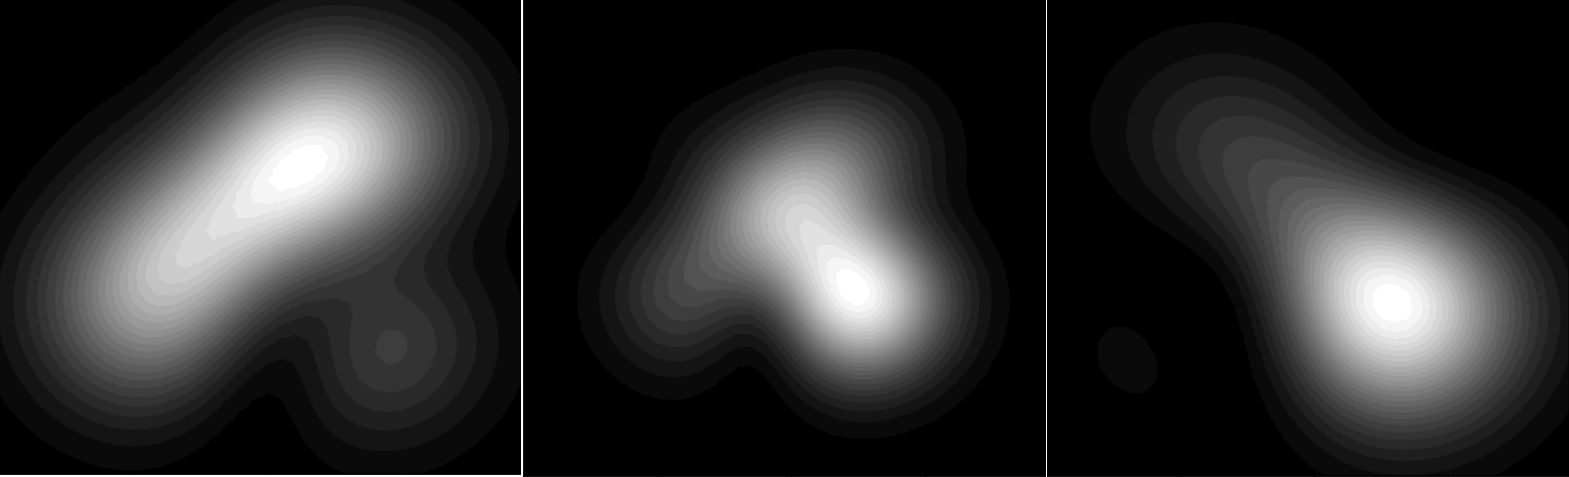
\includegraphics[width=6.00in]
{hermite-gauss/hermite-gauss.png}\\
\caption[Superposition of the first four Hermite-Guass modes]{Superposition of the first four Hermite-Guass modes. the left image is 0.3 m downstream from the waist, the center image is at the waist, the right image is 0.3 m upstream from the waist.}
\label{hermite-gauss}
\end{figure} 
%----------------------------------------------------------------------------


%----------------------------------------------------------------------------
%----------------------------------------------------------------------------
%----------------------------------------------------------------------------
%----------------------------------------------------------------------------
%----------------------------------------------------------------------------
